\chapter{Procedure}

\section{Resistor Network Calculation}

\begin{figure}[h]
    \centering
    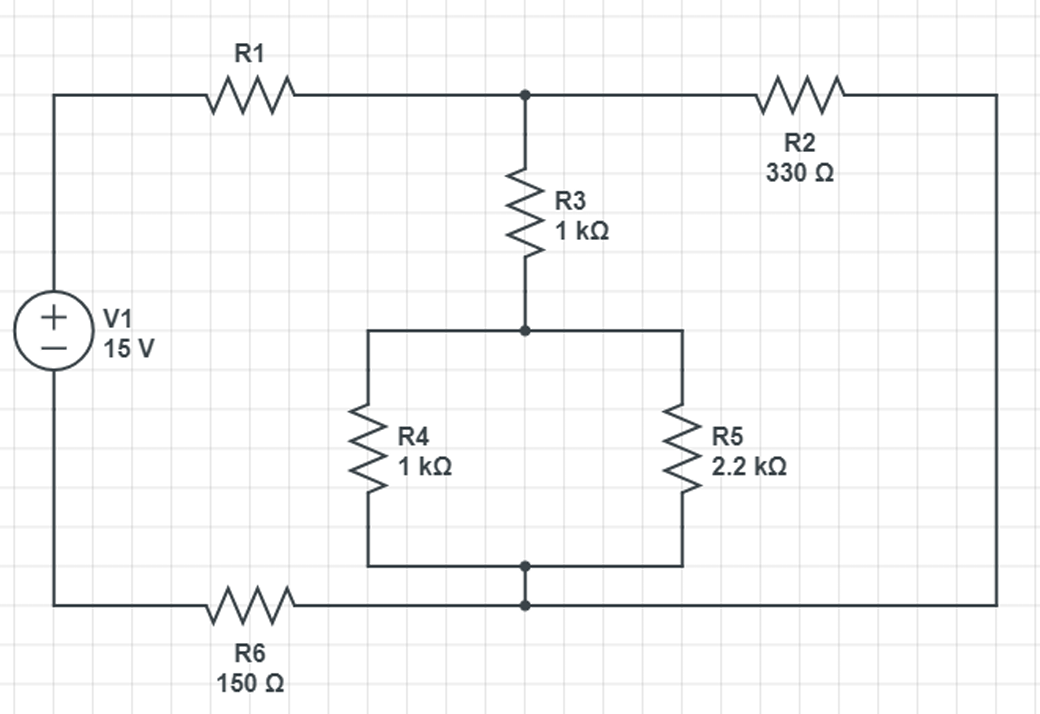
\includegraphics[width=0.7\textwidth]{assets/p1-circuit-scheme.png}
    \caption{Resistor Network}
    \label{fig:resistor_network}
\end{figure}

To find the $R_1$ value, we can divide total voltage to total current and find the equivalent resistance. Then we can find the $R_1$ value by using the equivalent resistance:

\begin{align*}
    \frac{V_{total}}{I_{total}} &= R_{eq} \\
    I_{total} &= I_1 + I_2 \\
    I_2 = \frac{3.8}{1k} &= 3.8\times 10^{-3}A \\
    I_1 = \frac{R_{345}}{R_2}\times I_2 &= \frac{1687.5}{330}\times 3.8\times 10^{-3}A \\
    I_{total} &= \frac{5111}{2.2\times 10^5}A \\
\end{align*}

\newpage
\thispagestyle{plain}

\begin{align*}
    R_{eq} &= \frac{15}{\frac{5111}{2.2\times 10^5}}\Omega \\
    &= \frac{3.3\times10^6}{5111}\Omega \\
    R_1 + 150 &+ \frac{1687.5\times 330}{1687.5 + 330} = \frac{3.3\times10^6}{5111}\Omega \\
    \implies R_1 &\approx 219.644\Omega \\
\end{align*}

\begin{figure}[h]
    \centering
    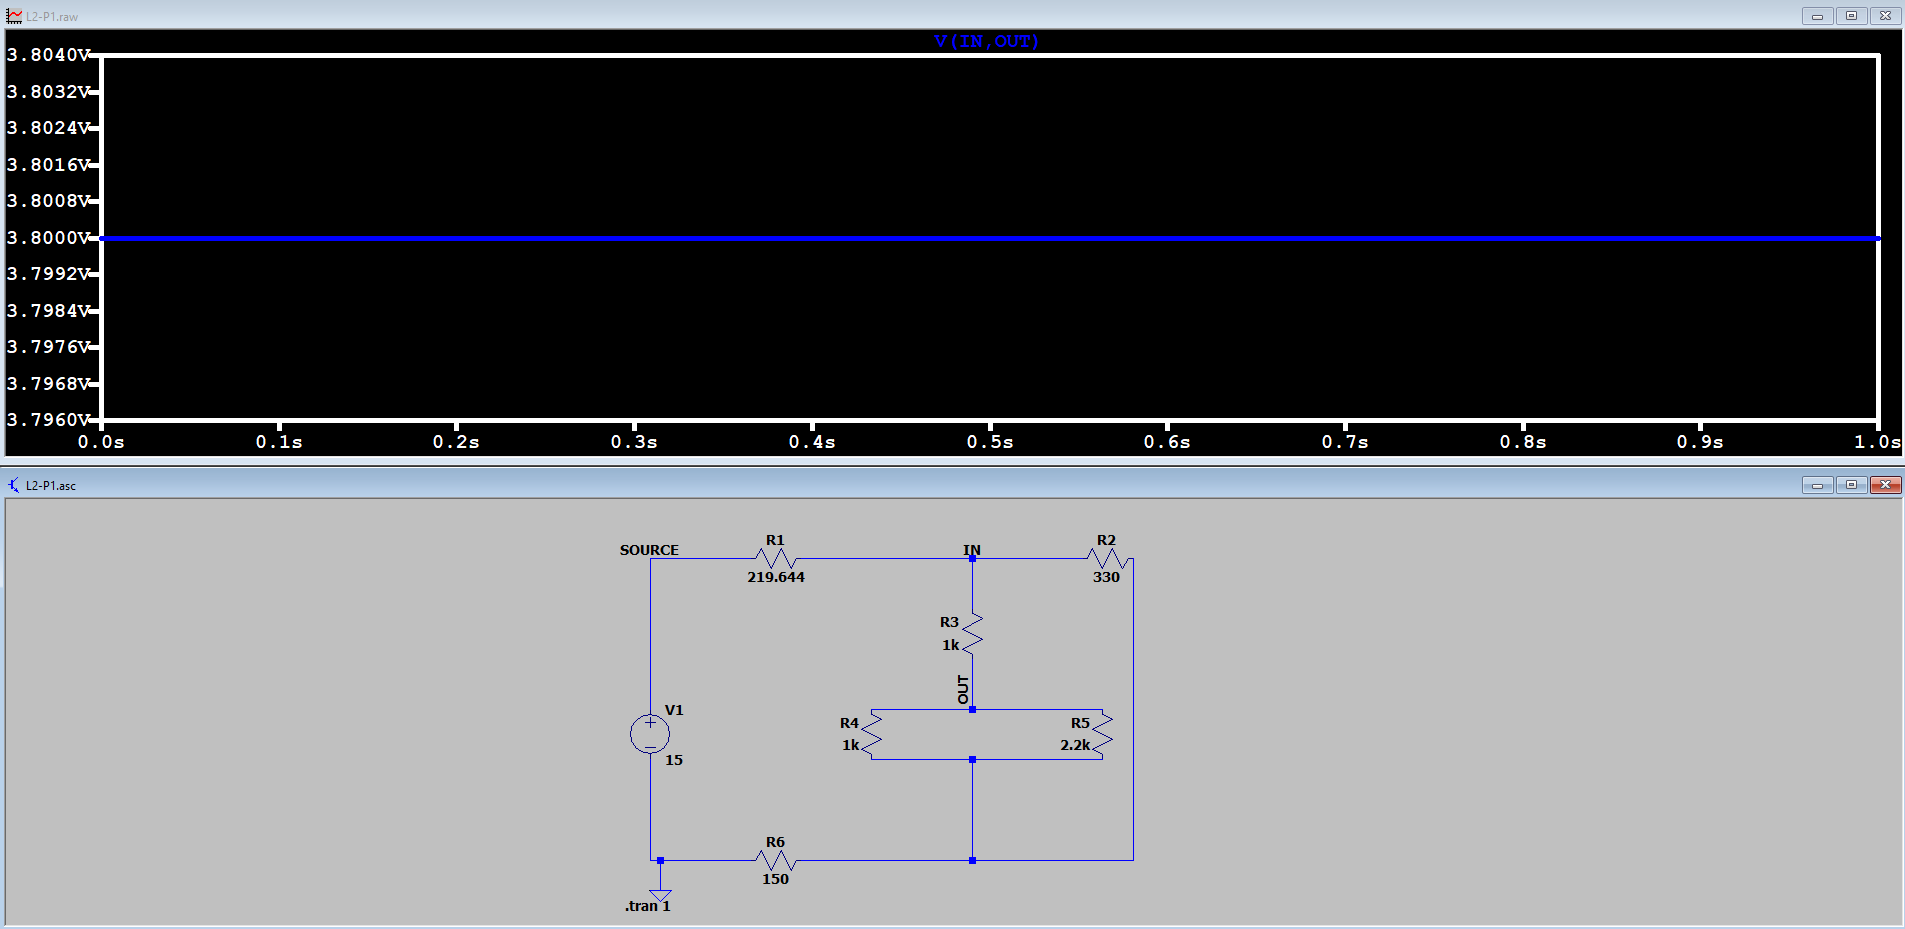
\includegraphics[width=1\textwidth]{assets/p1-res.png}
    \caption{$219.644\Omega$ Resistor Result}
    \label{fig:p1_result}
\end{figure}

After calculations, $R_1$ value is found as $219.644\Omega$. The simulation results are matching with the calculated results. The voltage on the $R_3$ resistor is $3.8V$ as expected.

\begin{table}[h]
    \centering
    \begin{tabular}{|l|l|l|}
        \hline
        \textbf{Resistor} & \textbf{Voltage} & \textbf{Current} \\ \hline
        $R_1$              & 5.1027V          & 23.2318mA        \\ \hline
        $R_2$              & 6.4124V          & 19.4318mA        \\ \hline
        $R_3$              & 3.7999V          & 3.7999mA         \\ \hline
        $R_4$              & 2.6124V          & 2.6124mA         \\ \hline
        $R_5$              & 2.6124V          & 1.1874mA         \\ \hline
        $R_6$              & 3.4847V          & 23.2318mA        \\ \hline
    \end{tabular}
    \caption{Voltage/Current over Resistors}
\end{table}

\newpage
\thispagestyle{plain}

\section{RC Circuit Phase Shift Analysis}

\begin{figure}[h]
    \centering
    \begin{circuitikz}
        \draw (0,0) to[vsourcesin, l={$V=5V_{pp}@50Hz$}] (0,3)
        to[R, l={$R=3.3k\Omega$}] (3,3)
        to[C, l={$C=1\mu F$}] (3,0)
        -- (0,0);
    \end{circuitikz}
    \caption{Simple RC Circuit}
    \label{fig:simple_rc_circuit}
\end{figure}

\begin{figure}[h]
    \centering
    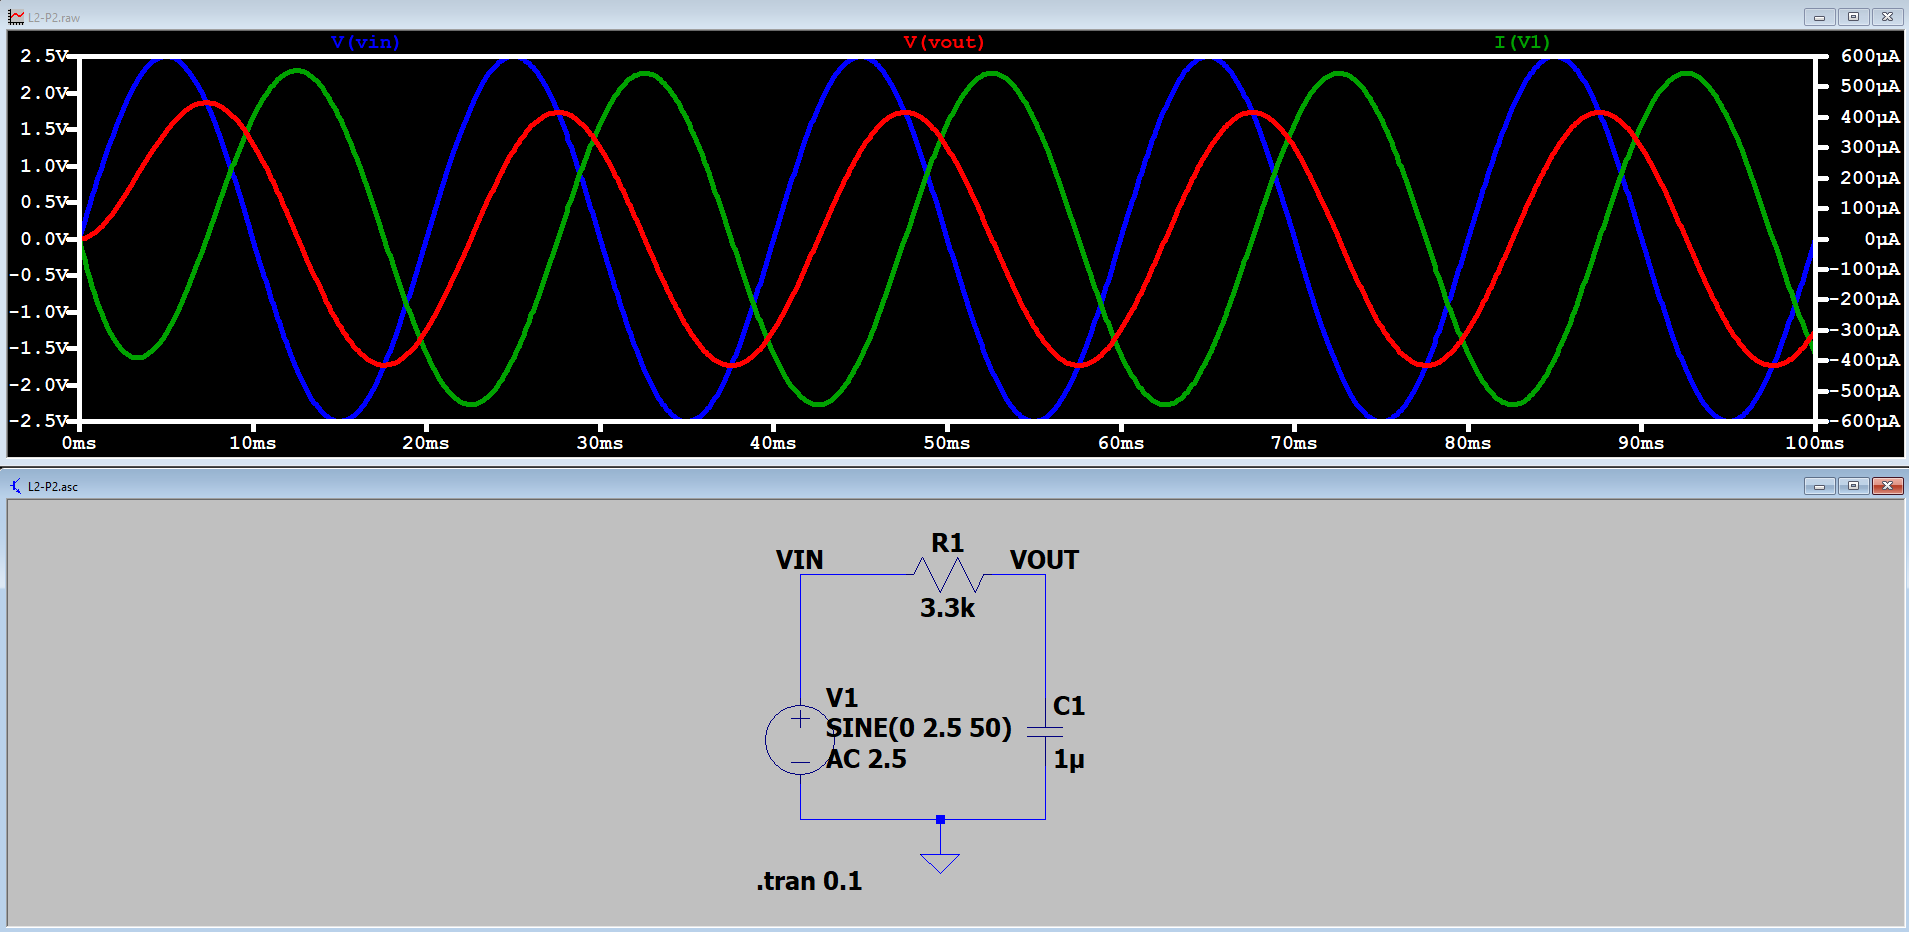
\includegraphics[width=1\textwidth]{assets/p2-circuit.png}
    \caption{RC Circuit Graph}
    \label{fig:rc_circuit_graph}
\end{figure}


In order to find the phase shift of the RC circuit, we need to find the impedance of the resistor and capacitor. The impedance of the resistor is $R$ and the impedance of the capacitor is $\frac{1}{j\omega C}$. The total impedance of the circuit is the sum of the impedance of the resistor and the impedance of the capacitor. The phase shift of the circuit is $\phi_{Z_{eq}} - 90^{\circ}(\text{phase angle of $\sin$})$:

\begin{align*}
    Z_{R} &= R \\
    Z_{C} &= \frac{1}{j\omega C} \\
    Z_{total} = Z_{R} + Z_{C} &= R + \frac{1}{j\omega C} = R + \frac{1}{j2\pi f C} \\
    \phi = \arctan\left(\frac{\Im(Z_{total})}{\Re(Z_{total})}\right) &= \arctan\left(\frac{\frac{1}{2\pi f C}}{R}\right) \\
    &\boxed{\phi = \arctan\left(\frac{1}{2\pi f R C}\right)}
\end{align*}

\newpage
\thispagestyle{plain}

\begin{figure}[h]
    \centering
        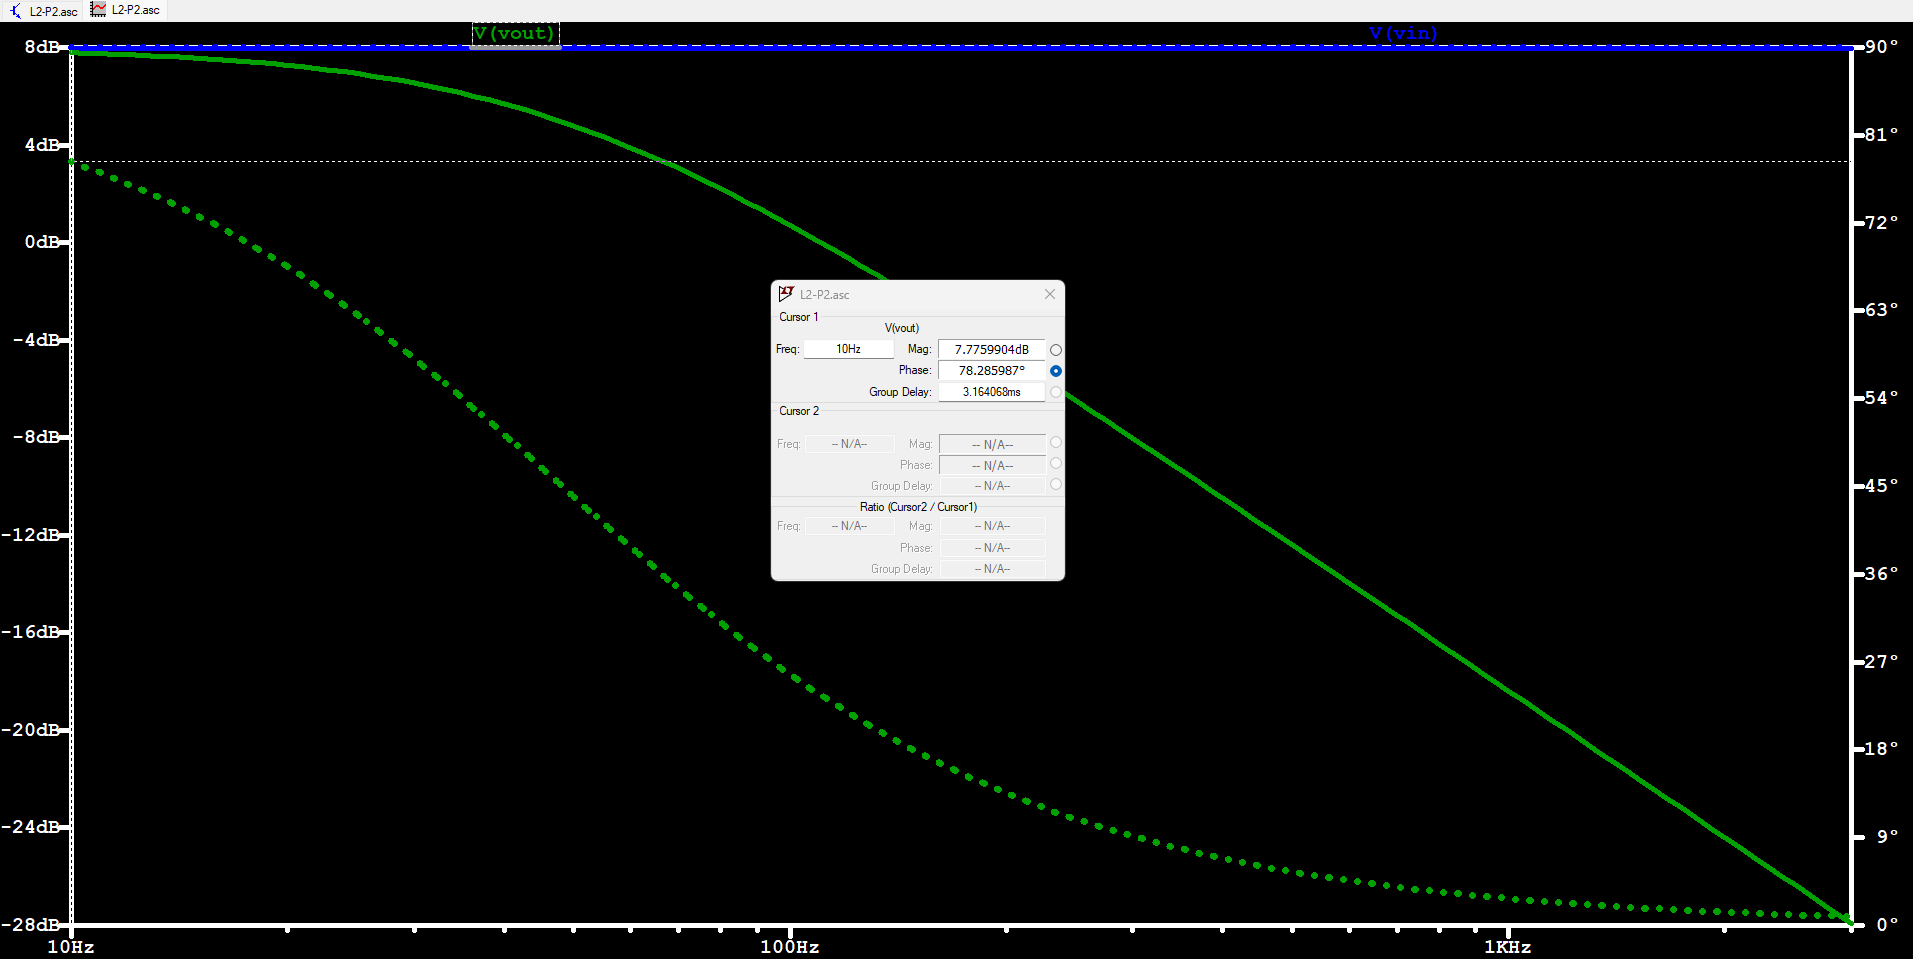
\includegraphics[width=0.6\linewidth]{assets/pd-10.png}
        \caption{$10Hz$ Phase Output}
        \label{fig:p2-10}
\end{figure}

\begin{figure}[h]
    \centering
        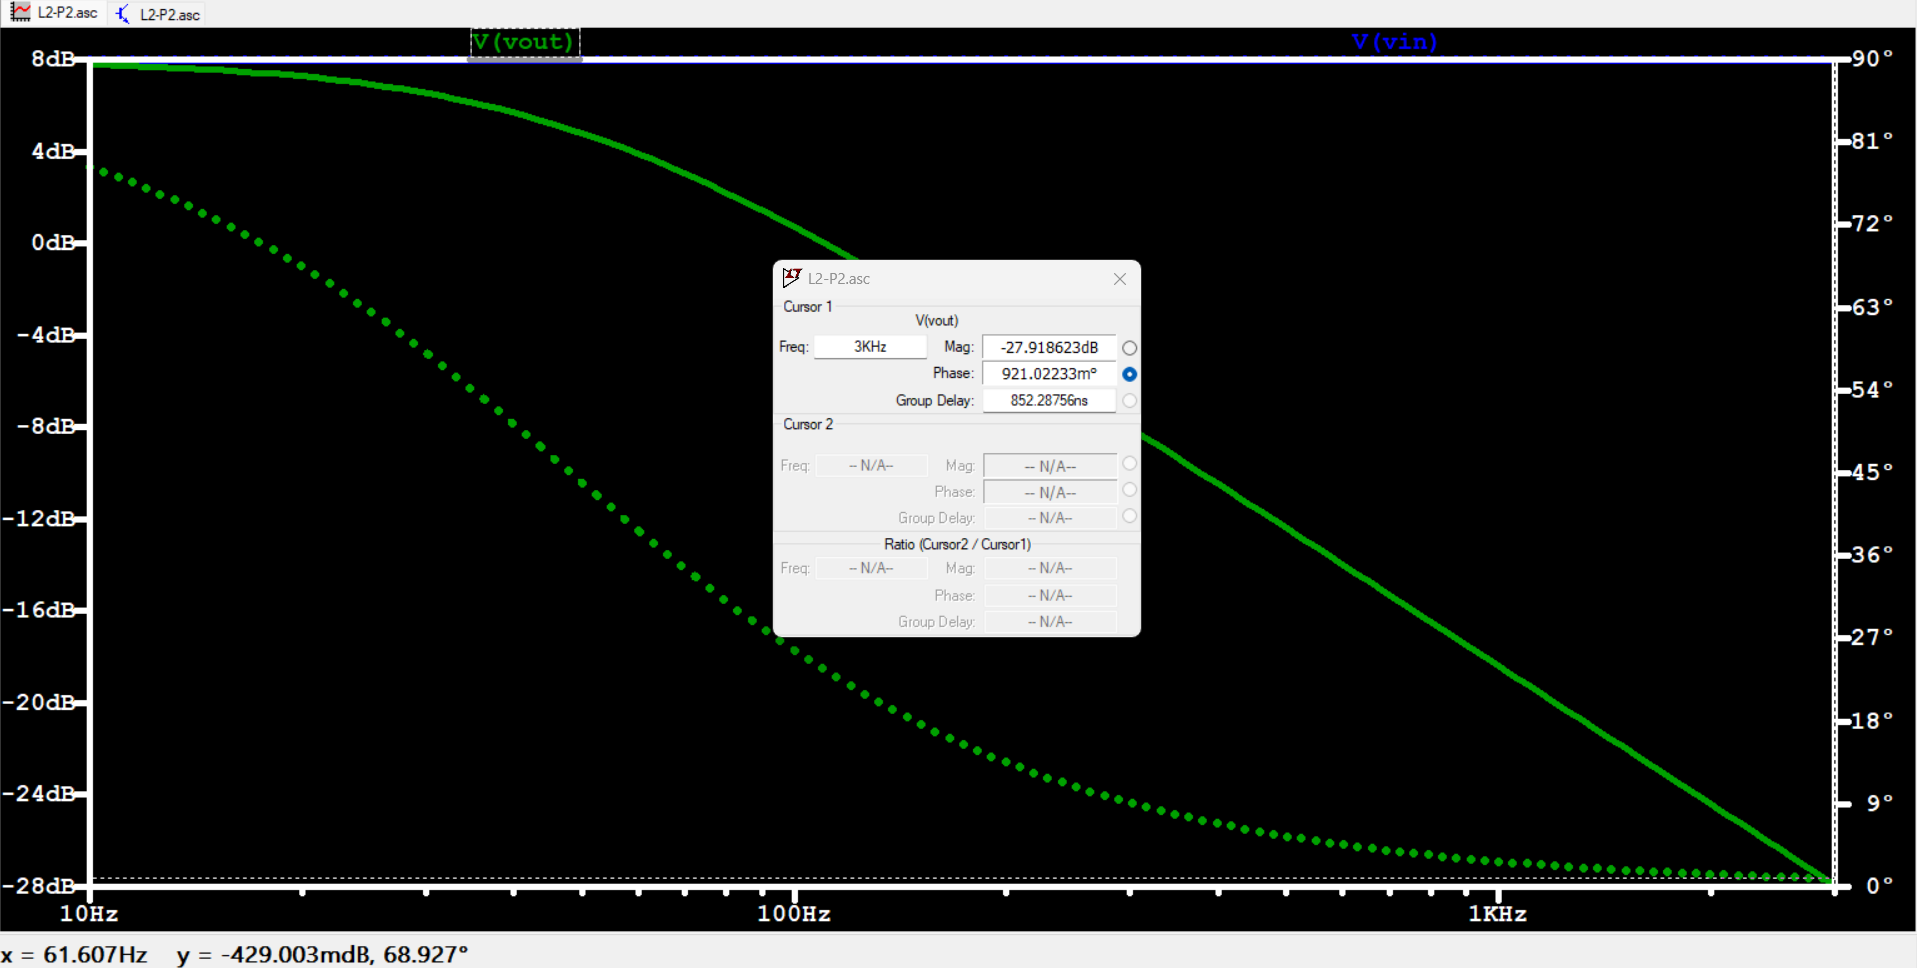
\includegraphics[width=0.6\linewidth]{assets/pd-3k.png}
        \caption{$3kHz$ Phase Output}
        \label{fig:p2-3k}
\end{figure}

\begin{table}[h]
    \centering
    \begin{tabular}{|l|l|l|l|}
        \hline
        \textbf{Frequency} & \textbf{Calculated Phase} & \textbf{Simulated Phase} & \textbf{Phase Shift} \\ \hline
        10Hz                 & $78.2859^{\circ}$           & $78.285987^{\circ}$      & $-11.714013   ^{\circ}$                          \\ \hline
        30Hz                 & $58.11^{\circ}$             & $58.11595^{\circ}$       & $-31.88405    ^{\circ}$                      \\ \hline
        50Hz                 & $43.96^{\circ}$             & $43.9667^{\circ}$        & $-46.0333     ^{\circ}$                  \\ \hline
        100Hz                & $25.74^{\circ}$             & $25.747201^{\circ}$      & $-64.252799   ^{\circ}$                      \\ \hline
        300Hz                & $9.13^{\circ}$              & $9.1330658^{\circ}$      & $-80.8669342  ^{\circ}$                       \\ \hline
        1kHz                 & $2.76^{\circ}$              & $2.7611528^{\circ}$      & $-87.2388472  ^{\circ}$                     \\ \hline
        3kHz                 & $921.02m^{\circ}$           & $921.02233m^{\circ}$     & $-89.078978   ^{\circ}$                    \\ \hline
    \end{tabular}
    \caption{Phase Angle Analysis}
\end{table}

Calculated and simulated results are matching. The phase angle of the circuit is increasing as the frequency increases. The phase angle of the circuit is almost $90^{\circ}$ at $3kHz$. This is expected because at higher frequencies, capacitor can not fully charge and discharge.

